\documentclass[11pt,aspectratio=169,xcolor=dvipsnames]{beamer}

% PACKAGES
\usepackage{amsmath}
\usepackage{amssymb}
\usepackage{graphicx}
\usepackage{hyperref}
\usepackage{bbm}
\usepackage[style=ieee]{biblatex}

\addbibresource{bibliography.bib}

\hypersetup{pdfborderstyle={/S/U/W 1}}

% THEME for uWaterloo slides %

% Credit to Junan Lin <junan_lin@hotmail.com> for the theme
\mode<presentation>{\setbeamercovered{invisible}
\usetheme{Madrid}
}
\usefonttheme{professionalfonts}

% Customize for Waterloo theme (gold and black)
\definecolor{UWgold}{RGB}{254,209,66} % Waterloo gold
\definecolor{darkgrey}{RGB}{169,169,169} 

\setbeamercolor{palette primary}{bg=black,fg=UWgold}
\setbeamercolor{palette secondary}{bg=white,fg=black}
\setbeamercolor{palette tertiary}{bg=UWgold,fg=white}
\setbeamercolor{palette quaternary}{bg=Black,fg=white}
\setbeamercolor{structure}{fg=darkgrey} % itemize, enumerate, etc
\setbeamercolor{section in toc}{fg=black} % TOC sections
\setbeamercolor{subsection in head/foot}{bg=UWgold,fg=white}

% Modify the default footer for better ratio
\makeatletter
\setbeamertemplate{footline}{%
  \leavevmode%
  \hbox{%
    \begin{beamercolorbox}[wd=.2\paperwidth,ht=2.5ex,dp=1.125ex,leftskip=.3cm]{author in head/foot}%
      \usebeamerfont{author in head/foot}\insertshortauthor, \insertshortinstitute
    \end{beamercolorbox}%
    \begin{beamercolorbox}[wd=.6\paperwidth,ht=2.5ex,dp=1.125ex,center]{title in head/foot}%
      \usebeamerfont{title in head/foot}\insertshorttitle
    \end{beamercolorbox}%
    \begin{beamercolorbox}[wd=.2\paperwidth,ht=2.5ex,dp=1.125ex,rightskip=.3cm plus1fil]{date in head/foot}%
      \usebeamerfont{date in head/foot}\hfill\insertshortdate\hfill\insertframenumber/\inserttotalframenumber
    \end{beamercolorbox}%
  }%
  \vskip0pt%
}
\makeatother

\setbeamertemplate{navigation symbols}{}
\setbeamerfont{footnote}{size=\tiny}

\title{Aerial Ad-hoc Network Formation using Differential Games}
\subtitle{Game-Theoretic Control Methods for UAV Swarms}

\author{Matteo Golin}
\date{April 2, 2026}

\institute[UWaterloo]
{University of Waterloo, Waterloo, ON, Canada\\
\medskip
\texttt{mgolin@uwaterloo.ca}
}

\logo{
\includegraphics[width=.25\paperwidth]{UniversityOfWaterloo_logo_horiz_rgb}}

\include{shorthands}

% DOCUMENT BEGINS

\begin{document}

\begin{frame}
    \titlepage
\end{frame}

\begin{frame}{Table of Contents}
    \tableofcontents
\end{frame}

% MOTIVATION
\section{Motivation}
% GUIDING QUESTIONS:
%
% What specific problem does your project address, and why is it important?

\begin{frame}{Motivation}
    \huge
    \centering
    Motivation
\end{frame}

\begin{frame}{Aerial Networks}
    \begin{columns}
        \column{0.5\textwidth}
        \begin{itemize}
            \item Flying base stations for 5G/6G applications are popular
                  \cite[12518]{drone-cells}
            \item High line of sight = better transmission, can relay data \cite{lora-drones}
            \item Deployable, dynamic traffic alleviation \cite{drone-cells}

        \end{itemize}

        \column{0.5\textwidth}
        \begin{figure}
            \centering
            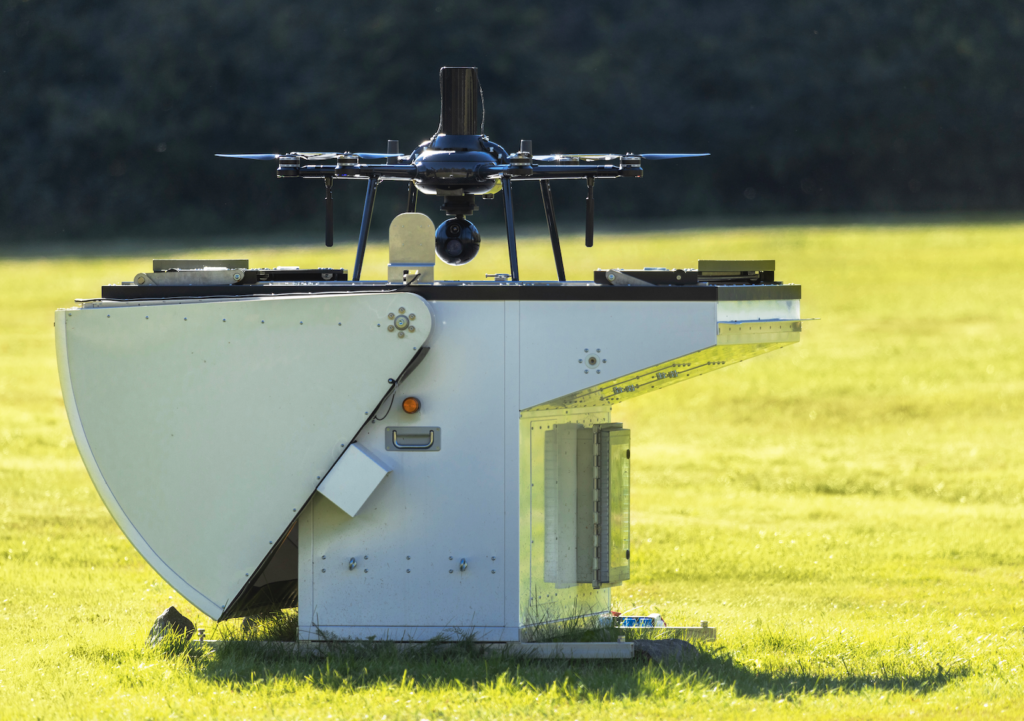
\includegraphics[width=0.75\linewidth]{assets/nokia-drone-network.png}
            \caption{"Drone in a box" from Nokia's 5G drone network platform
                \cite{img:nokia-drone}}
        \end{figure}
    \end{columns}

    % In recent years, mobile aerial networks have been of interest for 5G networking
    % due to the high line-of-sight transmission points available with aerial base
    % stations \cite[12518]{drone-cells}. Aerial networks are composed of multiple
    % aerial robots (often drones \cite[12518]{drone-cells}) which are deployed to
    % relieve traffic loads on existing base stations \cite{drone-cells}, form ad-hoc
    % networks and act as gateways between other networked devices.
    % \cite{lora-drones}

\end{frame}

\begin{frame}{Disaster Relief}

    \begin{columns}
        \column{0.35\textwidth}
        \begin{itemize}
            \item Beyond 5G networking: search \& rescue
            \item Mobile (in motion) networks
            \item Replacement for missing/damaged infrastructure
        \end{itemize}

        \column{0.65\textwidth}
        \begin{figure}
            \centering
            \subfloat[Coastguard flood response in Louisiana \cite{img:coast-guard}]{
                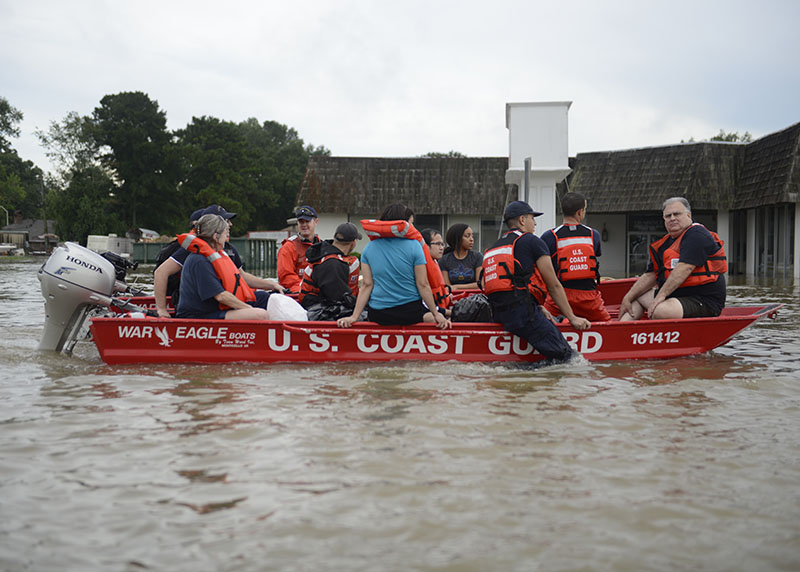
\includegraphics[width=0.4\linewidth]{assets/coastguard.jpeg}
            }
            \subfloat[Flood in Pigeon Hole, Australia \cite{img:rooftop-flood}]{
                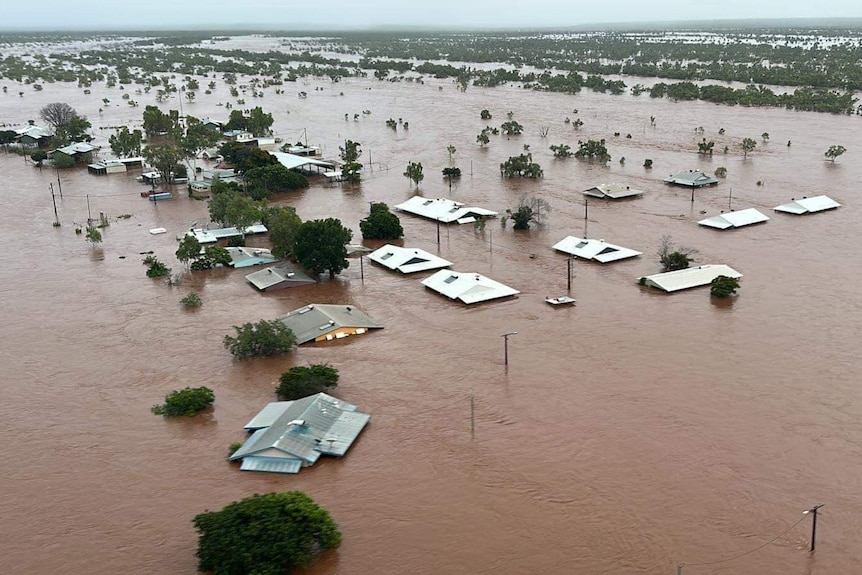
\includegraphics[width=0.4\linewidth]{assets/rooftop-flood.jpg}
            }
            \hspace*{\fill}
            \newline
            \subfloat[Rescue of 4 children in Amazon rainforest \cite{img:operation-hope}]{
                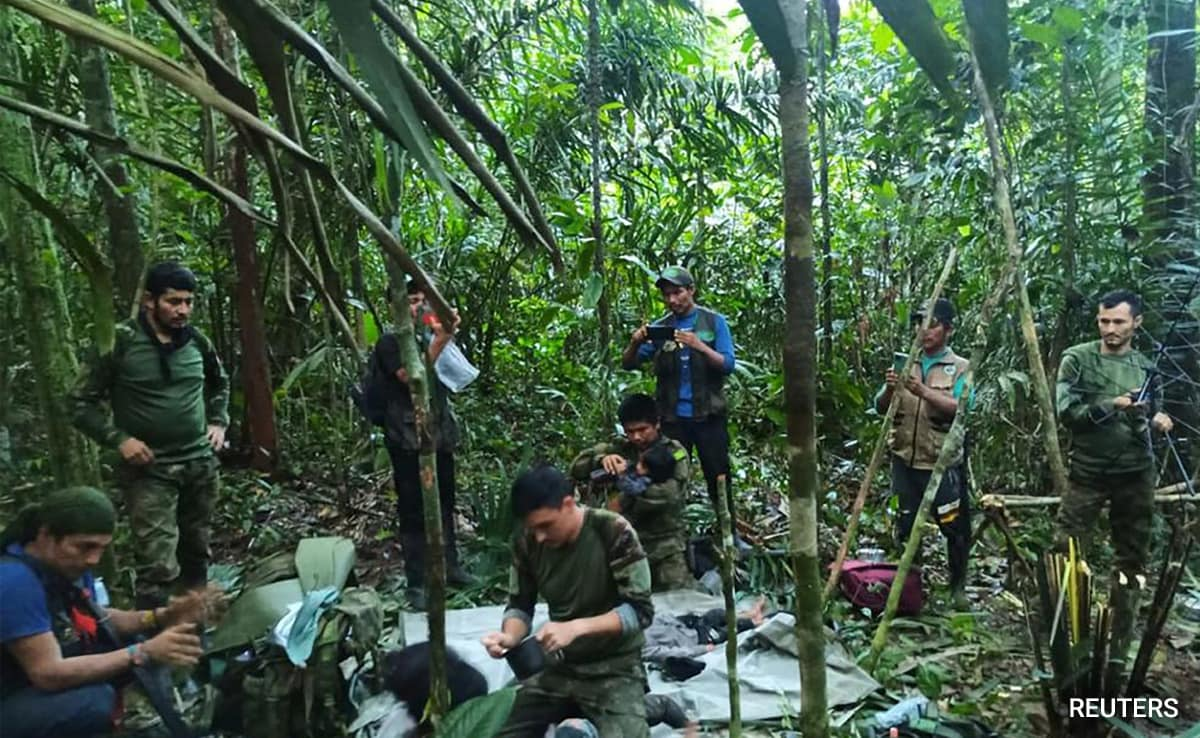
\includegraphics[width=0.4\linewidth]{assets/operation-hope.jpg}
            }
            \hspace*{\fill}
        \end{figure}
    \end{columns}

    % However, aerial networks have additional applications beyond 5G/6G commercial
    % networks. Ad-hoc aerial networks can be used in search-and-rescue or military
    % operations where there is a need for communication links between mobile ground
    % agents during missions.
\end{frame}

\begin{frame}{Application}
    \begin{columns}
        \column{0.5\textwidth}
        \begin{itemize}
            \item Deploy aerial network to connect multiple ground agents
            \item Ground agents move independently
            \item UAVs with radio equipment form ad-hoc network that responds to ground agent
                  movement
        \end{itemize}

        \column{0.5\textwidth}
        \begin{figure}
            \centering
            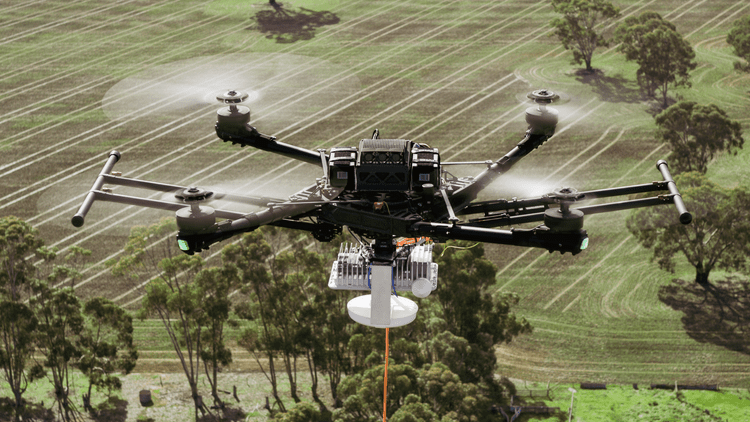
\includegraphics[width=0.75\textwidth]{assets/drone-base-station.png}
            \caption{A commercial drone carrying radio equipment \cite{img:drone-bs}}
        \end{figure}
    \end{columns}
\end{frame}


% LITERATURE REVIEW
\section{Existing Solutions}
\include{sections/literature}

% SETUP
\section{Problem Setup}
\include{sections/setup}

% CONTRIBUTION
\section{Contribution}
\include{sections/contribution}

% RESULTS
\section{Results}
% GUIDING QUESTIONS:
%
% What are the key artifacts of your project (e.g., methodology, hardware
% design, software algorithm, optimization or control technique)?
%
% How are these artifacts implemented and evaluated?
%
% What are your most important empirical or theoretical results?

\begin{frame}{Results}
    \huge
    \centering
    Results
\end{frame}

\begin{frame}{Simulating}
    \begin{columns}
        \column{0.5\textwidth}
        \begin{itemize}
            \item Created a simulation program using symbolic expression library
                  \texttt{symengine.py} \cite{symengine}
            \item Ran 20 simulations for varying $n$, $m$ using random initial conditions
            \item Pursuers strictly faster than evaders, and evaders following random walk
            \item Wrote data analysis script \& a C visualization engine \cite{diffgames}
        \end{itemize}

        \column{0.5\textwidth}
        \begin{figure}
            \centering
            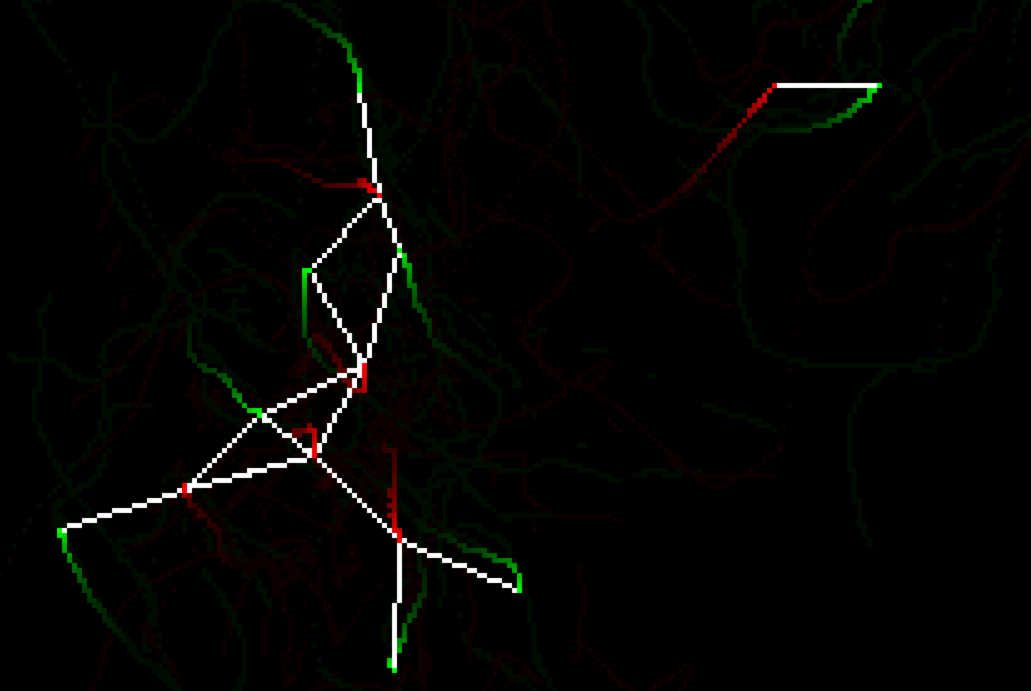
\includegraphics[width=0.75\linewidth]{assets/n10m10_graph.png}
            \caption{Interesting network formation with $n = m = 10$}
        \end{figure}
    \end{columns}
\end{frame}

% TODO: include videos of these?

\begin{frame}{$m = 2$ chains}
    \begin{figure}
        \subfloat[Random initial positions]{
            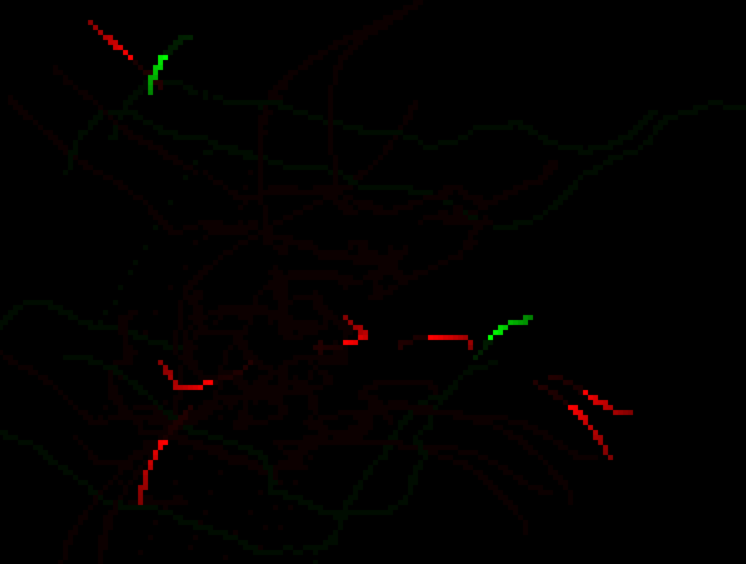
\includegraphics[width=0.4\textwidth]{assets/n8m2_initial_pos.png}
        }
        \subfloat[Chain formation connecting all agents]{
            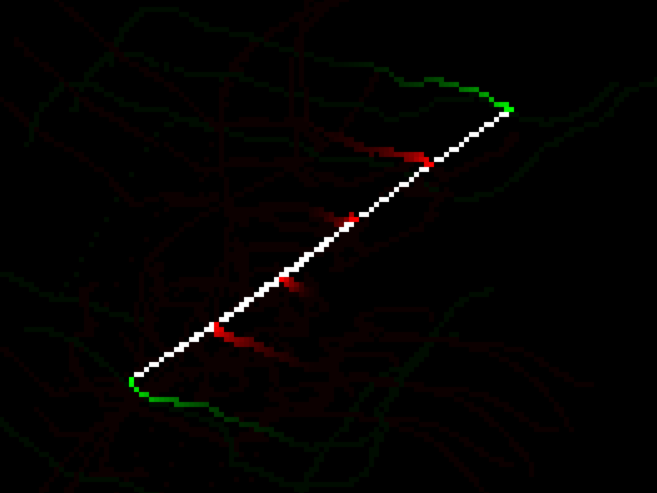
\includegraphics[width=0.4\textwidth]{assets/n8m2_chain.png}
        }
        \caption{Simulations with $m = 2$ form a chain for optimal connectivity (pictured $n = 8$)}
    \end{figure}
    {\tiny Pursuers in red, evaders in green, connections in white.
    Visualization from a bird's eye view.}
\end{frame}

\begin{frame}{Pursuer grouping for large $n$}
    \begin{figure}
        \subfloat[Random initial positions converging to group]{
            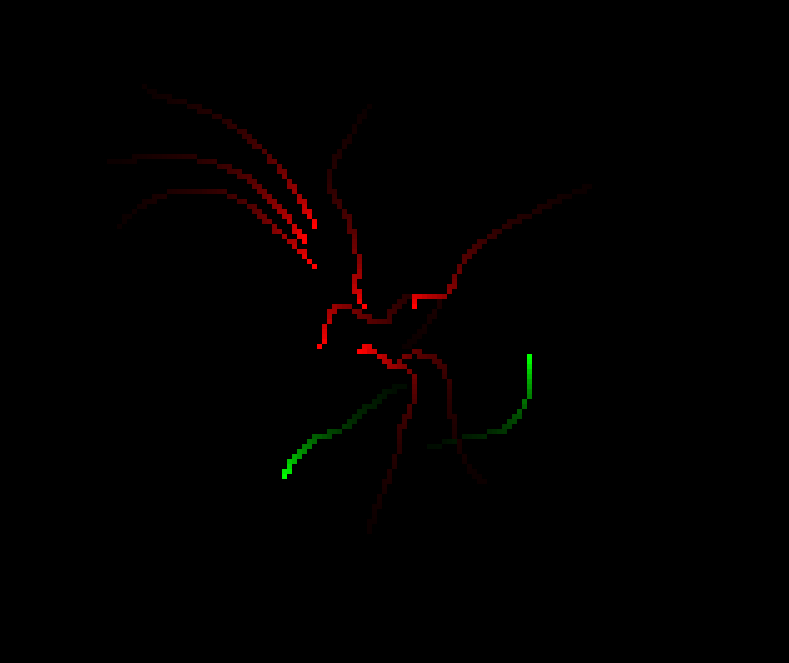
\includegraphics[width=0.3\textwidth]{assets/n8m2_cluster_start.png}
        }
        \subfloat[Tight grouping]{
            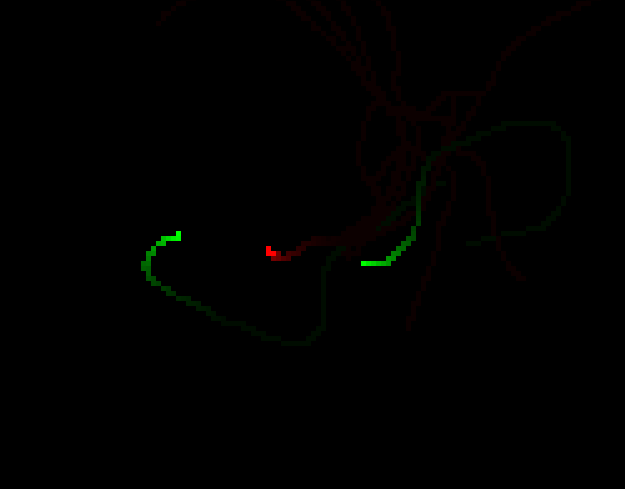
\includegraphics[width=0.3\textwidth]{assets/n8m2_cluster_tight.png}
        }
        \subfloat[Failure to split into full chain]{
            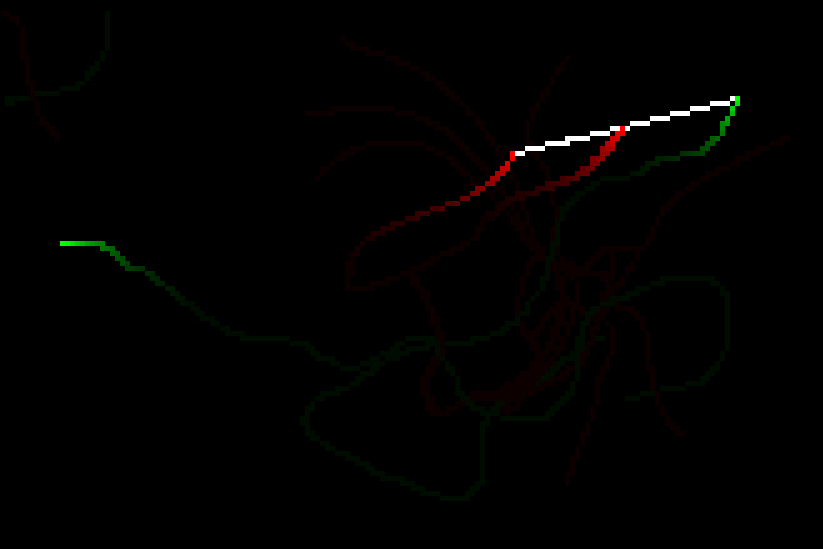
\includegraphics[width=0.3\textwidth]{assets/n8m2_cluster_end.png}
        }
        \caption{Pursuers cluster to maximize connectivity but are reluctant to separate later}
    \end{figure}
\end{frame}

\begin{frame}{Connectivity Analysis}
    \small
    \begin{columns}
        \column{0.5\textwidth}
        \begin{table}
            \begin{tabular}{cccl}
                \hline
                $n$ & $m$ & \% of duration connected & $\bar{\lambda_2}$ \\
                \hline
                1   & 1   & 96.51 \%                 & 1.807             \\
                1   & 2   & 28.48 \%                 & 0.158             \\
                1   & 3   & 11.44 \%                 & 0.041             \\
                2   & 2   & 46.05 \%                 & 0.364             \\
                3   & 3   & 44.97 \%                 & 0.162             \\
                4   & 4   & 40.00 \%                 & 0.191             \\
                5   & 5   & 33.90 \%                 & 0.060             \\
                6   & 1   & 99.69 \%                 & 6.230             \\
                6   & 2   & 64.59 \%                 & 0.923             \\
                6   & 3   & 52.99 \%                 & 0.341             \\
                6   & 4   & 33.18 \%                 & 0.102             \\
                6   & 5   & 33.58 \%                 & 0.083             \\
                6   & 6   & 34.58 \%                 & 0.072             \\
            \end{tabular}
        \end{table}
        \column{0.5\textwidth}
        \begin{table}
            \begin{tabular}{cccl}
                \hline
                $n$ & $m$ & \% of duration connected & $\bar{\lambda_2}$ \\
                \hline
                7   & 3   & 44.69 \%                 & 0.286             \\
                7   & 4   & 42.77 \%                 & 0.156             \\
                7   & 5   & 39.40 \%                 & 0.108             \\
                7   & 6   & 37.69 \%                 & 0.089             \\
                7   & 7   & 35.21 \%                 & 0.060             \\
                8   & 1   & 99.48 \%                 & 7.414             \\
                8   & 2   & 59.04 \%                 & 1.288             \\
                8   & 3   & 44.62 \%                 & 0.307             \\
                8   & 4   & 37.85 \%                 & 0.085             \\
                8   & 5   & 46.72 \%                 & 0.156             \\
                8   & 6   & 32.07 \%                 & 0.084             \\
                8   & 7   & 40.78 \%                 & 0.082             \\
                8   & 8   & 31.16 \%                 & 0.054             \\
            \end{tabular}
        \end{table}
    \end{columns}
    Disconnected at $\lambda_2 \le 10^{-2}$.
\end{frame}

\begin{frame}{Connectivity Analysis}
    \begin{figure}
        \subfloat[$\bar{\lambda_2}$ at each time step for 20 simulations of $n = 6, m = 3$]{
            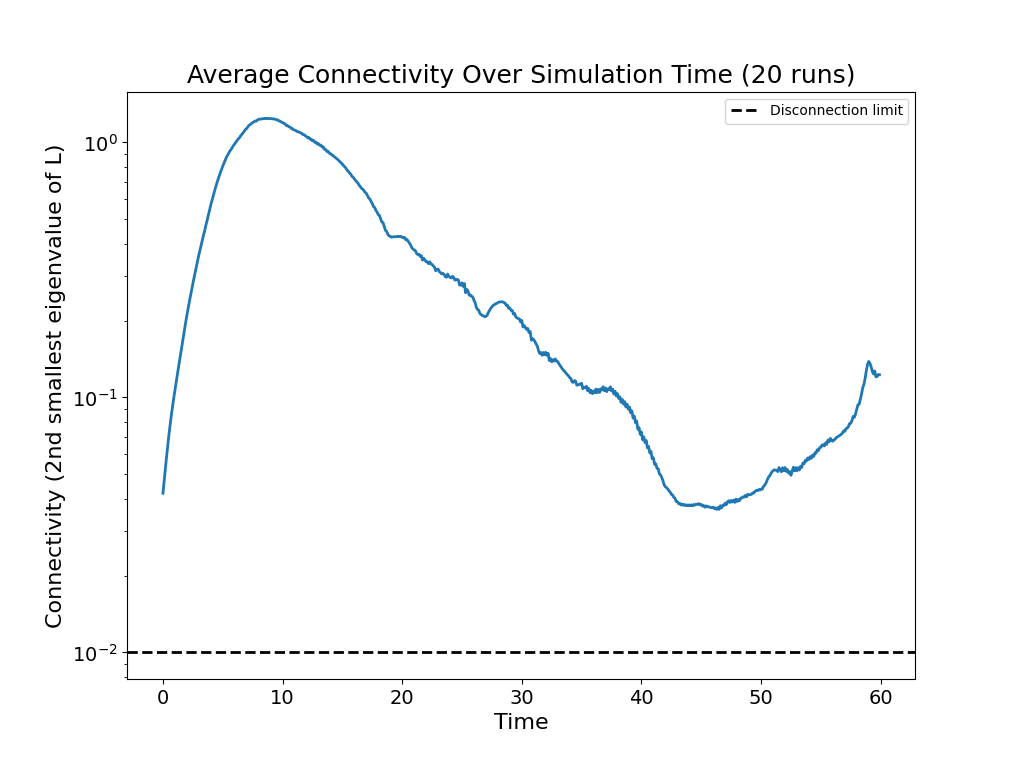
\includegraphics[width=0.45\textwidth]{assets/n6-eig.png}
        }
        \subfloat[$\bar{\lambda_2}$ at each time step for 20 simulations of $n = 8, m = 3$]{
            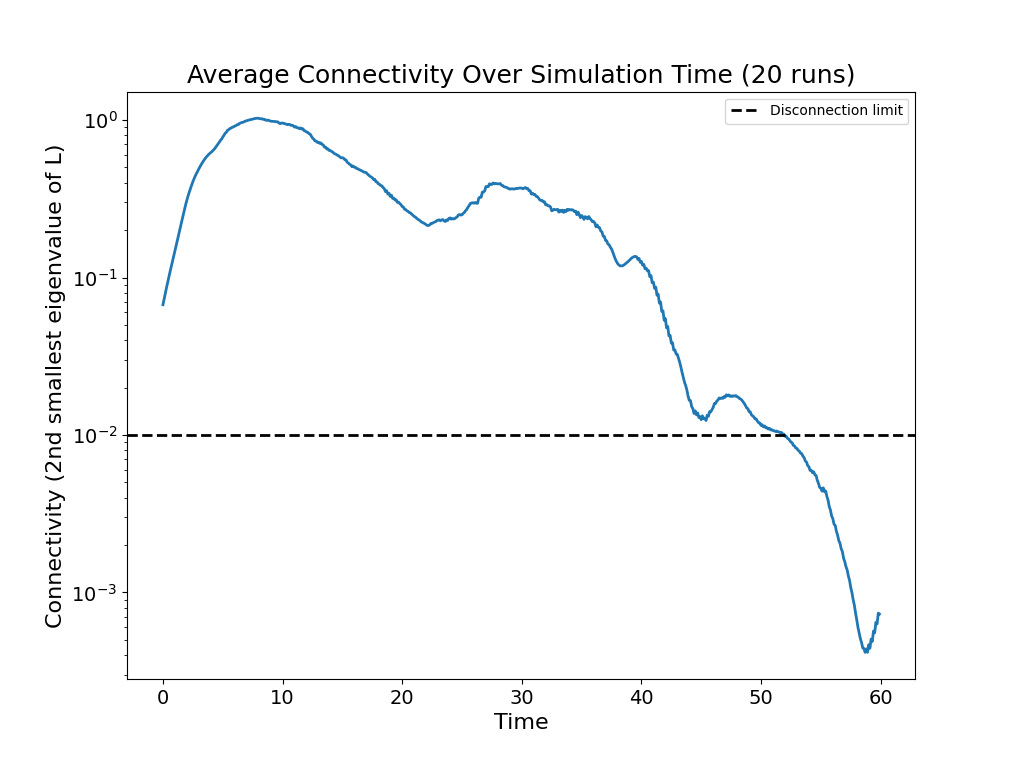
\includegraphics[width=0.45\textwidth]{assets/n8-eig.png}
        }
    \end{figure}
    Grouping behaviour affects connectivity trends. Evaders diffuse out over
    time.
\end{frame}


\section{Conclusion}

\begin{frame}{Conclusion}
    TODO
\end{frame}

\begin{frame}
    \centering
    \LARGE Thank you!
\end{frame}

\section*{References}

\begin{frame}[allowframebreaks]{References}
    \printbibliography
\end{frame}

\appendix

\begin{frame}{Visualization Software}
    The program used to visualize the results of these simulations can be found on
    GitHub at
    \href{https://github.com/linguini1/diffgames}{\texttt{linguini1/diffgames}}.
    The module under \texttt{replay/} was specifically used to replay simulation
    files generated by the simulation program.
\end{frame}

% TODO: include agent dynamics, path loss model, and etc.


\end{document}
